% Compile using: TEXINPUTS=minted/source: pdflatex -shell-escape %
\documentclass[12pt,utf8,notheorems,compress,t]{beamer}
\usepackage{etex}

\usepackage[english]{babel}

\usepackage{mathtools}
\usepackage{booktabs}
\usepackage{array}
\usepackage{ragged2e}
\usepackage{multicol}
\usepackage{tabto}
\usepackage{xstring}
\usepackage{mathtools}
\usepackage{soul}\setul{0.2ex}{}
\usepackage[all]{xy}
\xyoption{rotate}
\usepackage{tikz}
\usetikzlibrary{calc,shapes.callouts,shapes.arrows}

\usepackage[protrusion=true,expansion=true]{microtype}

\newcommand{\NN}{\mathbb{N}}
\renewcommand{\_}{\mathpunct{.}}
\newcommand{\?}{\,{:}\,}
\newcommand{\defeq}{\vcentcolon=}
\newcommand{\defeqv}{\vcentcolon\equiv}

\setlength\parskip{\medskipamount}
\setlength\parindent{0pt}

\title{Konstruktive Mathematik, die Doppelnegationsübersetzung und Continuations}
\author{Ingo Blechschmidt}
\date{4. Dezember 2015}

\usetheme{Warsaw}
\usecolortheme{seahorse}
%\usefonttheme{default}?
%\usepackage{kurier}?
\usefonttheme{serif}
\usepackage{libertine}
%\usepackage{mathpazo}
\useinnertheme{rectangles}

\setbeamertemplate{blocks}[rounded][shadow=false]

\newenvironment{changemargin}[2]{%
  \begin{list}{}{%
    \setlength{\topsep}{0pt}%
    \setlength{\leftmargin}{#1}%
    \setlength{\rightmargin}{#2}%
    \setlength{\listparindent}{\parindent}%
    \setlength{\itemindent}{\parindent}%
    \setlength{\parsep}{\parskip}%
  }%
  \item[]}{\end{list}}

\newcommand{\pointthis}[2]{%
  \tikz[remember picture,baseline]{\node[anchor=base,inner sep=0,outer sep=0]%
    (#1) {#1};\node[overlay,rectangle callout,%
    callout relative pointer={(-0.2cm,0.8cm)},fill=blue!20] at ($(#1.north)+(1.8cm,-1.4cm)$) {#2};}%
}%

\newcommand{\hcancel}[5]{%
  \tikz[baseline=(tocancel.base)]{
    \node[inner sep=0pt,outer sep=0pt] (tocancel) {#1};
    \draw[red, line width=0.4mm] ($(tocancel.south west)+(#2,#3)$) -- ($(tocancel.north east)+(#4,#5)$);
  }%
}

\newcommand{\slogan}[1]{%
  \begin{center}%
    \setlength{\fboxrule}{0pt}%
    \setlength{\fboxsep}{-14pt}%
    {\usebeamercolor[fg]{item}\fbox{\usebeamercolor[fg]{normal
    text}\parbox{0.9\textwidth}{\begin{center}#1\end{center}}}}%
  \end{center}%
}

\setbeamertemplate{frametitle}[default][colsep=-2bp,rounded=false,shadow=false,center]
\setbeamertemplate{frametitle}{%
  \vskip1em%
  \leavevmode%
  \begin{beamercolorbox}[dp=1ex,center]{}%
      \usebeamercolor[fg]{item}{\textbf{\Large \insertframetitle}}
  \end{beamercolorbox}%
}


\setbeamertemplate{headline}{}
\setbeamertemplate{navigation symbols}{}

\newcounter{framenumberpreappendix}
\newcommand{\backupstart}{
  \setcounter{framenumberpreappendix}{\value{framenumber}}
}
\newcommand{\backupend}{
  \addtocounter{framenumberpreappendix}{-\value{framenumber}}
  \addtocounter{framenumber}{\value{framenumberpreappendix}} 
}

\setbeamertemplate{footline}{%
  \begin{beamercolorbox}[wd=\paperwidth,ht=2.5ex,dp=1.25ex,right,rightskip=1mm,leftskip=1mm]{frametitle right}
    {\quad} \inserttitle \hfill \insertauthor \quad
    \insertframenumber\,/\,\inserttotalframenumber {\quad}
  \end{beamercolorbox}}

\newcommand{\hil}[1]{{\usebeamercolor[fg]{item}{\textbf{#1}}}}

\IfSubStr{\jobname}{\detokenize{nonotes}}{
  \setbeameroption{hide notes}
}{
  \setbeameroption{show notes}
}
\setbeamertemplate{note page}[plain]

\begin{document}

\begin{frame}[c]
  \centering
  
\includegraphics[scale=0.5]{images/fortune-teller}
  \medskip

  \hil{Konstruktive Mathematik, \\ die Doppelnegationsübersetzung und Continuations}
  \medskip

  \scriptsize
  Ingo Blechschmidt \\
  Universität Augsburg
  \medskip

  Haskell in Leipzig \\
  4. Dezember 2015
  \par
\end{frame}


\section{Konstruktive Mathematik}

\subsection{Das Axiom vom ausgeschlossenen Dritten}

\begin{frame}\frametitle{Nichtkonstruktive Beweise}
  Eine Zahl heißt genau dann \hil{rational}, wenn sie sich als Bruch zweier
  ganzer Zahlen schreiben lässt.
  \begin{itemize}
    \item $\frac{21}{13}$ und $37$ sind rational.
    \item $\sqrt{2}$ und $\pi$ sind irrational.
  \end{itemize}

  \only<1>{\vspace*{1em}\centering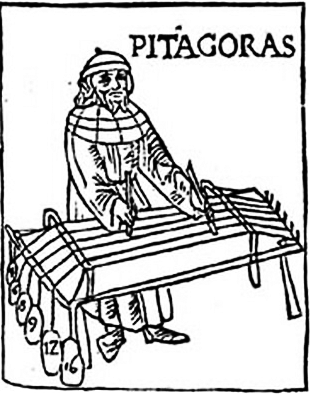
\includegraphics[scale=0.3]{images/pythagoras}}

  \pause

  \hil{Satz.} Es gibt \hil{irrationale} Zahlen~$x$ und~$y$ sodass~$x^y$ rational ist.
  \medskip

  \pause
  \hil{Beweis.} Entweder ist~$\sqrt{2}^{\sqrt{2}}$ rational oder nicht.
  \begin{enumerate}
    \item Im ersten Fall sind wir fertig.
    \item Im zweiten Fall können wir~$x \defeq \sqrt{2}^{\sqrt{2}}$ und~$y \defeq
  \sqrt{2}$ nehmen. Dann ist~$x^y = \sqrt{2}^{\sqrt{2} \cdot \sqrt{2}} =
  \sqrt{2}^2 = 2$ rational.
  \end{enumerate}
\end{frame}

\end{document}
